% =====================================================================
%  Seance 2 -- D. TP du brut au dataset supervise + synthese
% =====================================================================
\section{TP « Du brut au dataset supervisé » et synthèse}

\begin{frame}{Le TP : objectif final, un jeu de données supervisé}
\footnotesize%
\begin{columns}[t]
\begin{column}{0.52\textwidth}
\begin{kbox}[Ce que vous produisez à 18 h]
\begin{center}
\file{nosys\_features.csv}\\[1mm]
une ligne = (serveur, fenêtre de 10 min)\\[1mm]
\begin{tabular}{@{}l@{}}
\toprule
variables de niveau : cpu\_moy, ram\_moy\ldots\\
dispersion : cpu\_max, cpu\_amplitude\\
distribution : lat\_p99\\
dynamique : cpu\_delta (dérivée)\\
contexte : h\_sin, h\_cos, jour\_sem\\
\textbf{cible : incident\_30min} $\in \{0,1\}$\\
\bottomrule
\end{tabular}
\end{center}
\end{kbox}
\begin{ebox}[Chiffres attendus]
\textbf{34 560} fenêtres (8 serveurs $\times$ 4 320), dont
\textbf{120 positives} (\textbf{0,35 \%}) --- une classe \emph{très} rare,
c'est exactement ce que la séance 3 apprendra à traiter.
\end{ebox}
\end{column}
\begin{column}{0.44\textwidth}
\begin{center}
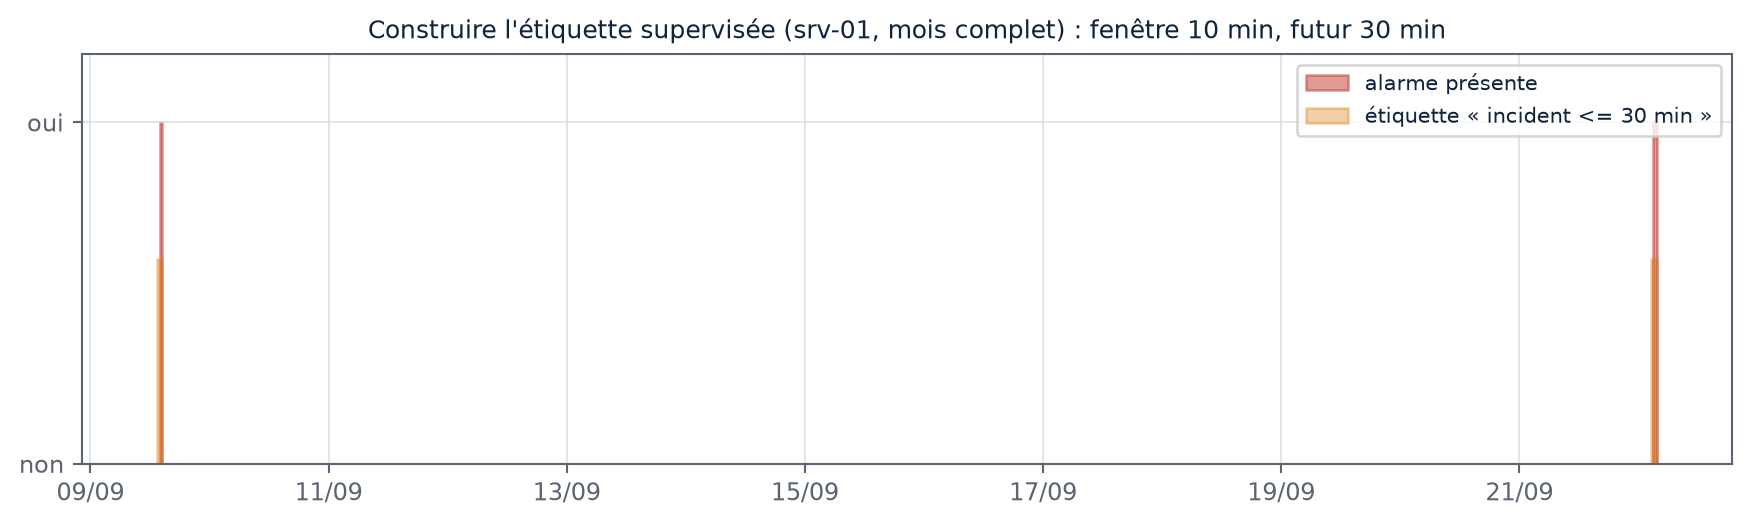
\includegraphics[width=\textwidth]{f15_etiquette.png}
\end{center}
\vspace{1mm}
\begin{wbox}[La règle anti-fuite]
Le calcul de \py{incident\_30min} utilise \textbf{uniquement} la colonne
\py{alarme} du futur. Les variables de signaux, elles, utilisent
\textbf{uniquement le passé} de la fenêtre. Mélanger les deux
$=$ tricher, et le modèle de la séance 3 paraîtra magique
en validation, nul en production.
\end{wbox}
\end{column}
\end{columns}
\end{frame}

\begin{frame}[fragile]{TP B1 --- audit des défauts (30 min)}
\begin{codebox}[B1. Compter, ne pas réparer encore]
\begin{lstlisting}
b = pd.read_csv("data/nosys_metriques_brutes.csv",
                parse_dates=["horodatage"])
b = b.sort_values(["serveur", "horodatage"]).reset_index(drop=True)

print("doublons :", b.duplicated().sum())          # 200
print("NaN par colonne :")
print(b[["cpu_pct","ram_pct","latence_ms",
         "paquets_perdus_pct","temperature_c"]].isna().sum())
print("valeurs impossibles :")
print("cpu > 100 :", (b["cpu_pct"] > 100).sum())        # 4
print("temp > 80 :", (b["temperature_c"] > 80).sum())   # 5
print("points par serveur :")
print(b.groupby("serveur").size())                 # srv-07 a 2880
\end{lstlisting}
\end{codebox}
\begin{abox}[Livrable B1]
Un tableau d'audit : \textbf{chaque défaut, son volume, son hypothèse de cause}
(doublon réseau, capteur flottant, pic capteur, redémarrage d'agent,
config de granularité, dérive). \textbf{Avant de réparer, on explique.}
\end{abox}
\end{frame}

\begin{frame}[fragile]{TP B2 --- nettoyage (35 min)}
\footnotesize%
\begin{codebox}[B2. Réparer dans le bon ordre]
\begin{lstlisting}
# 1. dedoublonner
b = b.drop_duplicates()

# 2. erreurs physiquement impossibles -> NaN (pas de suppression !)
b.loc[b["cpu_pct"] > 100, "cpu_pct"] = np.nan
b.loc[b["temperature_c"] > 80, "temperature_c"] = np.nan

# 3. grille explicite 5 min par serveur (les trous -> NaN visibles)
def sur_grille(g):
    g = g.set_index("horodatage").drop(columns=["serveur"])
    return g.reindex(pd.date_range(g.index.min(), g.index.max(),
                                   freq="5min"))
b = b.groupby("serveur", group_keys=False).apply(sur_grille)

# 4. imputation courte (<= 2 pas), tendance-compatible
b = b.interpolate(limit=2, limit_direction="both")
\end{lstlisting}
\end{codebox}
\begin{columns}[t]
\begin{column}{0.48\textwidth}
\begin{wbox}[Pourquoi « NaN » et pas « suppression »]
Supprimer une ligne d'incident suspecte, c'est supprimer
\textbf{l'exemple le plus précieux} du dataset. On neutralise
l'erreur de mesure, on garde l'observation.
\end{wbox}
\end{column}
\begin{column}{0.48\textwidth}
\begin{ebox}[Contrôle de sortie B2]
Après B2 : 0 doublon, 0 CPU $>$ 100, 0 NaN résiduels
(interpolation a couvert les trous courts), 8 serveurs
sur la même grille --- srv-07 inclus.
\end{ebox}
\end{column}
\end{columns}
\end{frame}

\begin{frame}[fragile]{TP B3 --- construire les signaux (30 min)}
\begin{codebox}[B3. Fenêtre de 10 min, par serveur]
\begin{lstlisting}
f = (b.reset_index().set_index("horodatage")
      .groupby("serveur")
      .resample("10min")
      .agg(cpu_moy=("cpu_pct", "mean"),
           cpu_max=("cpu_pct", "max"),
           ram_moy=("ram_pct", "mean"),
           lat_moy=("latence_ms", "mean"),
           lat_p99=("latence_ms", lambda s: s.quantile(0.99)),
           perte_moy=("paquets_perdus_pct", "mean"),
           temp_moy=("temperature_c", "mean")))

# dynamique : derivee du CPU (fenetre precedente)
f["cpu_delta"] = f.groupby("serveur")["cpu_moy"].diff()

# contexte : encodage cyclique
h = f.index.get_level_values("horodatage").hour
f["h_sin"] = np.sin(2*np.pi*h/24)
f["h_cos"] = np.cos(2*np.pi*h/24)
\end{lstlisting}
\end{codebox}
\begin{abox}[Exercice bonus B3]
Détecter la dérive de srv-06 : régression de \py{temp\_moy} sur le temps
(\py{np.polyfit}) par fenêtre de 7 jours. Vous devez retrouver la pente
d'env. \textbf{+0,22 °C/jour} mesurée en cours.
\end{abox}
\end{frame}

\begin{frame}[fragile]{TP B4 --- l'étiquette « incident $\le$ 30 min » (35 min)}
\begin{codebox}[B4. Regarder le futur avec la colonne alarme --- et SEULEMENT elle]
\begin{lstlisting}
# alarme par fenetre de 10 min (max des 2 sous-fenetres de 5 min)
al = (b.reset_index()
       .groupby(["serveur", pd.Grouper(key="horodatage", freq="10min")])
       ["alarme"].max().unstack(0))          # fenetres x serveurs

# max sur les 3 fenetres qui suivent (t+10, t+20, t+30 min)
fut = al.copy()
for k in (1, 2, 3):
    fut |= al.shift(-k)

# on aplatit : une ligne = (fenetre, serveur)
fut = fut.stack().rename("incident_30min")
features = f.join(fut).dropna(subset=["incident_30min"])
print(features["incident_30min"].value_counts())
# -> 1 : 120   (0,35 %)   0 : 34 440
\end{lstlisting}
\end{codebox}
\begin{wbox}[Deux questions de contrôle à se poser]
\begin{enumerate}
\item Pourquoi \py{shift(-k)} et pas \py{shift(+k)} ? (réponse : regarder
le \textbf{futur}, pas le passé.)
\item Où la fuite serait-elle possible ici ? (réponse : nulle part ---
\py{alarme} n'entre PAS dans les features, seulement dans la cible.)
\end{enumerate}
\end{wbox}
\end{frame}

\begin{frame}{TP B5 --- livrable et barème}
\begin{columns}[t]
\begin{column}{0.52\textwidth}
\begin{abox}[À rendre]
\begin{enumerate}
\item \textbf{\file{nosys\_features.csv}} --- le dataset supervisé complet
(34 560 lignes, $\approx$ 12 colonnes).
\item \textbf{Dictionnaire des variables} --- une ligne par colonne :
définition, fenêtre de calcul, unité, méthode (ex. : « lat\_p99 :
quantile 0,99 de latence sur fenêtre 10 min, ms »).
\item \textbf{Note de 5 lignes} sur les choix : quelle imputation, pourquoi ;
quelles bornes physiques ; ce que vous avez exclu et pourquoi.
\end{enumerate}
\end{abox}
\end{column}
\begin{column}{0.44\textwidth}
\begin{kbox}[Barème (20 pts)]
\begin{itemize}
\item Audit des défauts complet et expliqué --- 4 pts
\item Nettoyage correct (ordre, bornes physiques) --- 5 pts
\item Signaux corrects (fenêtres, p99, cyclique) --- 4 pts
\item Étiquette sans fuite --- \textbf{5 pts} (la note la plus chère :
c'est là que 80 \% des projets échouent)
\item Dictionnaire et reproductibilité --- 2 pts
\end{itemize}
\end{kbox}
\end{column}
\end{columns}
\end{frame}

\begin{frame}{Quiz de synthèse --- 5 questions (10 min)}
\begin{qbox}[Répondez seul(e), puis correction]
\begin{enumerate}
\item Pourquoi trier par (serveur, temps) AVANT les fenêtres glissantes ?\\
(a) pour l'esthétique \quad (b) une moyenne mobile sur un ordre mélangé
est mathématiquement fausse \quad (c) pandas l'exige
\item CPU à 350 \% : erreur de mesure ou incident ? Et CPU à 96 \% pendant
un incident ?\\
(a) les deux sont des erreurs \quad (b) le premier est une erreur
(impossible), le second un événement réel à \textbf{garder} \quad (c) les
deux sont des incidents
\item Quelle est la part de fenêtres positives dans le dataset final ?\\
(a) 50 \% \quad (b) 5 \% \quad (c) 0,35 \%
\item La fuite de données dans B4 serait possible si\ldots\\
(a) on ajoutait \py{alarme} aux variables d'entrée \quad (b) on standardisait
après le split \quad (c) les deux
\item L'interpolation bat le forward-fill sur CPU car :\\
(a) elle est plus rapide \quad (b) le signal évolue en tendance --- erreur
0,74 contre 1,02 \quad (c) pandas la recommande
\end{enumerate}
\end{qbox}
\end{frame}

\begin{frame}{Corrigé du quiz de synthèse}
\begin{solbox}[Réponses justifiées]
\begin{enumerate}
\item \textbf{b} --- démontré en cours : la moyenne mobile suppose l'ordre
temporel ; sur des lignes mélangées elle mélange passé et futur.
\item \textbf{b} --- bornes physiques d'abord (règle métier), statistiques ensuite.
\item \textbf{c} --- 120 / 34 560 = 0,35 \% : c'est le défi de la séance 3
(classes très rares).
\item \textbf{c} --- les deux sont des fuites : l'une dans les features,
l'autre dans les statistiques de standardisation.
\item \textbf{b} --- mesuré : 0,743 contre 1,018 (erreur absolue moyenne sur
600 points masqués de srv-01).
\end{enumerate}
\end{solbox}
\begin{kbox}[Prochaine séance]
Séance 3 : avec ce dataset en main --- \textbf{anomalies (isolation forest)
et classification sur classe rare (0,35 \%)}, précision/rappel et seuils.
Votre \file{nosys\_features.csv} est la matière première.
\end{kbox}
\end{frame}
